\documentclass{llncs}
\usepackage[utf8]{inputenc}
\usepackage{amsmath}
\usepackage{graphicx}

\begin{document}
\pagestyle{headings}
\addtocmark{The difference operation between templates of binary cellular automata}

\title{The difference operation between templates of binary cellular automata}

\titlerunning{Difference operation between templates}

\author{Zorandir Soares\inst{2} \and Maurício Verardo\inst{2} \and
Pedro P. B. de Oliveira\inst{1}\inst{2}}

\authorrunning{Zorandir Soares, Maurício Verardo, and Pedro de Oliveira} 

\tocauthor{Zorandir Soares, Maurício Verardo, and Pedro de Oliveira}

\institute{Universidade Presbiteriana Mackenzie\\
Faculdade de Computação e Informática
\and
Pós-Graduação em Engenharia Elétrica e Computação\\
Rua da Consolação 896, Consolação\\
01302-907 São Paulo, SP - Brazil\\
\email{zorandir@gmail.com}\\
\email{mauricio.verardo@gmail.com}\\
\email{pedrob@mackenzie.br}}

\maketitle

\begin{abstract}
A cellular automata template is a generalisation of the state transition tables of cellular automata. Templates have recently been introduced to represent families of cellular automata that share a given property. This paper introduces the operation of difference between templates, used to find cellular automata that have a given property but lack another. We also introduce a process called \textit{exception templates} that is required to this operation. Experimental results of both techniques are illustrated with examples in the space of elementary cellular automata.
\keywords{Cellular automata, rule space, templates, difference between templates, exception templates.}
\end{abstract}

\section{Introduction}
\label{sec:introducao}
Cellular automata (CAs) are dynamical systems typically discrete in time, space and state variables.
CAs can produce behavior of great complexity even based on simple rules of local action \cite{wolfram2002}. The study of classical problems of cellular automata, like the parity problem \cite{Betel2013} and the density classification problem \cite{deOliveira2014density} can help understand how this complex behavior emerges.

The most basic approach to find a suitable solution to classic problems consists in testing each of the rules of a particular family of CAs in order to check whether some rule is able to solve the problem. However, this approach shows to be inefficient or impractical for larger families of CAs, which is the most usual panorama in literature.

Evolutionary computing has been consistently used to deal with larger families. This type of algorithm has proven very effective to find solutions for density and parity classification \cite{wolz2008very}.

Another strategy to find suitable rules is restricting the search space by rules that have a given property. In order to represent a subspace with a particular property without the need of enumerate all of the rules in the space, one can use \textit{templates}, as proposed by De Oliveira and Verardo  \cite{deOliveira2014,deOliveira2014b}.

Up to the moment, two key operations have been defined to be applied to templates: \textit{expansion} and \textit{intersection} \cite{deOliveira2014,deOliveira2014b}. Here we introduce two new operations, namely, the \textit{difference between templates} and another that generates the \textit{exception templates}. Moreover, application of these operations are presented with simple examples.

This paper is organised as follows. Next, Section \ref{sec:automatos_celulares} gives some basic concepts about cellular automata. Following, Section \ref{sec:templates} presents more details about templates and its major operations. Section \ref{sec:diferenca_entre_templates_e_templates_de_excecao} introduces the operation of difference between templates and the one that generates the \textit{exception templates}, as well as their applications. The paper concludes with Section \ref{sec:consideracoes_finais} with closing remarks.

\section{Cellular Automata}
\label{sec:automatos_celulares}
Cellular Automata are simple mathematical idealisations of natural systems \cite{wolfram1994cellular}. They consist of a lattice of discrete cells, each of which can take on one of a finite set of discrete states in a given time step. The states of the cells evolve in discrete time steps usually according to deterministic rules that specify the state of each cell according to those of their neighbouring cells \cite{wolfram1994cellular}.

We assume that the cells have $k$ possible states which are represented by integer values in the range of $[0, k-1]$. The state of a cell is changed by the local function of the automaton (its rule), formed by a state transition set, that applies to its current state and those of adjacent cells. In order to define the size of the neighbourhood of the cells, usually a radius $r$ is defined encompassing the extent by which the neighbouring cells will be accounted for.

A family (or space) of cellular automata, is defined by the radius $r$ and the number of states $k$. One-dimensional cellular automata with $r=1$ e $k=2$ constitute the so-called elementary cellular automata. In order to refer to the rules of a space, it is common to use the number obtained by the decimal representation of the outputs of the state transitions, sorting the neighbourhoods lexicographically from the largest to smallest state; for instance, in the elementary space, the number of the rules corresponds to the decimal sequence formed by the 8-bit output, arranged from neighbourhood 111 down to 000. 

\begin{figure}
  \centering
  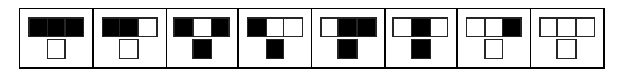
\includegraphics[width=0.9\textwidth]{Figure1.pdf}
  \caption{Rule table of the elementary CA 60.}
  \label{fig:table60}
\end{figure}

In other words, as neighbourhood are sets of adjacent cells that determine the state of the current cell in the next time step, all CA has a rule that relates each possible neighbourhood with the state of the central cell in the next time step. This rule can then be represented by rule tables with $n$-tuples, $n = 2r + 1$  in the one-dimensional case. For example, the rule table of the elementary CA 60 is given by 
((1,1,1),0), (1,1,0),0), (1,0,1),1), (1,0,0),1), (0,1,1),1), (0,1,0),1), (0,0,1),0), (0,0,0),0)), and illustrated in Figure \ref{fig:table60} by its iconic representation table of the elementary CA 60.

Since the number of rules in a space is given by $k^{k^{2r+1}}$, any increase in the values of $k$ and $r$ generates families with an exponentially increase in the number of rules. An approach to handle this problem is to use static properties as a hint on how the CA will behave during its evolution. A static property is obtained directly from the CA's rule table. The use of static properties can highly restrict the initial search space. With templates we can represent a set of rules with a certain static property. For the sake of simplicity, whenever we refer to a CA template from now on, we mean one-dimensional and binary CA template.

In order to explain how templates work, it is important to understand the properties of number conservation, internal symmetry and colour blindness, that will be used in later examples.

\subsection{Number Conservation, Internal Symmetry and Colour Blind Cellular Automata}
Number conservation is a static property that determines that the sum of the states of a particular cellular automata should not change during the CA's evolution, regardless of the initial configuration.

According to Boccara and Fukś \cite{boccara2002}, a CA is conservative when its local function $f$, applied to every neighbourhood $(\alpha_0,\alpha_1, \dots, \alpha_{n-1})$, considering $n=2r+1$, satisfies the conditions described in Eq. \ref{eq:conservativeCA}.
\begin{equation}
\begin{split}
f(\alpha_0,\alpha_1, \dots,\alpha_{n-1}) = \alpha_0 + (\sum_{i=0}^{n-2}f(0_0,0_1, \dots,0_i,\alpha_1,\alpha_2, \dots,\alpha_{n-1}) \\- f(0_0,0_1, \dots,0_i,\alpha_0,\alpha_1, \dots,\alpha_{n-i-1}))
\label{eq:conservativeCA}
\end{split}
\end{equation}

Another interesting property is internal symmetry. But in order to grasp its meaning, first we need the concept of rule equivalence. The following explanations are valid for binary rules, although it is possible to generalise the notion to arbitrary $k$ states.
  \begin{figure}
    \centering
    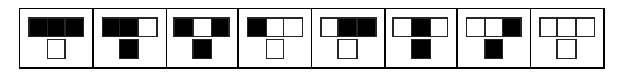
\includegraphics[width=0.9\textwidth]{Figure2.pdf}
    \caption{Elementary CA 102, equivalent by reflection to elementary CA 60.}
    \label{fig:table102}
  \end{figure}
  
Given the rule table of a CA, there are three transformations that can be applied to it, such that the resulting rule table represents an equivalent rule to the original CA: \textit{reflection}, \textit{conjugation} and \textit{composition}. Reflection is the transformation obtained by mirroring the bits of the neighbourhoods in all neighbourhoods of the rule table, while preserving the same output. Conjugation is obtained by flipping all states of the cells of the rule table. Finally, by composition we mean the mathematical notion of composing conjugation and reflection, regardless of the order. Figure \ref{fig:table102} illustrates the process; after applying the reflection transformation in elementary rule 60 we obtain the elementary CA 102.

The internal symmetry is defined by the number of state transitions that remains the same after a specific transformation has been applied. For example, the internal symmetry value by reflection of the elementary CA 60 is 4 because it shares the state transitions $((1,1,1),0)$, $((1,0,1),1)$, $((0,1,0),1)$ and $ ((0,0,0),0)$ with rule 102, its equivalent rule by reflection.

%\subsection{Colour blind cellular automata}
Finnaly, the colour blind property is directly related to transformation by conjugation, so that the colour blind rules are those with maximum internal symmetry by conjugation. Then, a CA is considered colour blind when it is invariant to the application of all state permutations in the states of transition table \cite{salo2013color}. Naturally, there is generally $k!$ permutations, but only one in the binary case, which can be described as $\{0 \to 1 ,\, 1 \to 0\}$.

\section{Templates}
\label{sec:templates}
A template is a generalisation of the state transition tables of CAs by means of variables or functions. A template represents a set of CAs which share a given static property. Templates were created and implemented by De Oliveira and Verardo \cite{deOliveira2014,deOliveira2014b} and are currently available in the open source library \textit{CATemplates} \cite{CATemplates} on GitHub.

Formally, a \textit{template} is an $n$-tuple formed by $k^{2r+1}$ items, wherein each item $i$ represents a function $g_i(x_{k^{2r+1}-1},x_{k^{2r+1}-2},\dots,x_1,x_0)$. By default, a template variable $x_i$ can take on any state between 0 and $k-1$, but their values can be limited by the notation $x_i \in C$, in which $C$ is a set representing the possible values of $x_i$. %TODO verificar essa função $g_i$

As an example, the template of the elementary space $T_1 = (1,1,1,1,1-x_1,x_2,x_1,0)$ represents all rules that have state 0 at position 0 (always from right to left), state 1 at positions 4, 5, 6 and 7, any state in the interval $[0, k-1]$ at positions 1 and 2, and in position 3 the complementary state to the value of position 1. Therefore the template $T_1$ represents the set of elementary rules $\{248,242,252,246\}$, that correspond in binary form, respectively to $\{(1,1,1,1,1,0,0,0), (1,1,1,1,0,0,1,0), (1,1,1,1,1,1,0,0), (1,1,1,1,0,1,1,0)\}$.

The process of finding all the rules represented by a template is called \textit{expansion}. There are several generator algorithms of templates representing rules with certain property implemented in the library \textit{CATemplates} \cite{CATemplates}.

The template $T_{comp} = (1 - x_0, 1 - x_4, 1 - x_2, x_4, 1 - x_1, x_2, x_1, x_0)$ of the elementary CAs, for example, when expanded generates only rules that have maximum internal symmetry by reflection and by conjugation. But the template $T_{cb} = (1 - x_0, 1 - x_1, 1 - x_2, 1 - x_3, x_3, x_2, x_1, x_0)$ of the elementary CAs expands only to colour blind rules.

Besides the possibility of template expansion, De Oliveira and Verardo \cite{deOliveira2014,deOliveira2014b} also developed an algorithm to generate templates that represent the intersection between two sub-spaces of rules represented by distinct templates. To illustrate, consider the search for a rule set composed by CAs that are both colour blind and have maximum internal symmetry by composition of reflection and conjugation. In order to find this rule set, two steps need to be performed: first one must match the two templates that represent the desired properties, thus forming an equation system defined by the template components. Them by solving the equation system, relationships are generated between the variables that, when applied to templates received as input, will result in the template representing the intersection.

For instance, consider the template $T_{comp}$ representing rules with maximum symmetry by composition and the template $T_{cb}$ representing colour blind rules. The first step towards the intersection between the two template is to equate them, which leads to the equation system represented by Eq. \ref{eq:interseccaoP1}:
\begin{equation}
\left\{\begin{matrix}
1 - x_0 & = & 1 - x_0 \\
1 - x_4 & = & 1 - x_1 \\
1 - x_2 & = & 1 - x_2 \\
x_4   & = & 1 - x_3 \\
1 - x_1 & = & x_3   \\
x_2   & = & x_2   \\
x_1   & = & x_1   \\
x_0   & = & x_0   \\
\end{matrix}\right.
\label{eq:interseccaoP1}
\end{equation}

Then, the system is solved yielding the solution set $S = \{x_3 = 1-x1, x_4 = x_1\}$. This solution set is then applied as a set of replacements to the templates received as parameter. If the latter do not show variable constraints, the result of either replacements can be chosen, thus ending the process and resulting in the template $(1 - x_0, 1 - x_1, 1 - x_2, x_1, 1 - x_1, x_2, x_1, x_0)$; this template is the intersection of $T_{comp}$ and $T_{cb}$ and, therefore, represents all elementary rules that are colour blind and possess maximum symmetry by composition.

If at least one of the templates presents variables with restriction, a second step should be carried out. Therefore, the expressions that restrict the variables are extracted, generating a set that is then translated into a new equation system to be solved; the new solution set is then applied as a set of replacements in the templates passed as parameter.

Inspired by the intersection operation, here we introduce the operation of difference between templates.

\section{Difference Between Templates and Exception Templates}
\label{sec:diferenca_entre_templates_e_templates_de_excecao}

The difference operation has two templates as input parameters, which we call $T_{minuend}$ and $T_{subtrahend}$. The operation’s output results in a set of templates that represents all rules accounted for template $T_{minuend}$ but not by $T_{subtrahend}$.

The difference operation is a process with several steps. The first consists in the process of intersecting the two parameter templates, resulting in template $T_{int}$. If the intersection is null, the outcome of the difference is $T_{minuend}$ itself. Otherwise, it is matched to template $T_{minuend}$, thus generating logical combinations of equations. Then, the tautological equations, if any, are removed, and the remaining equations subjected to a negation operation, which in the binary case means the permutations $\rho = (0 \to 1, 1 \to 0)$. The existing occurrences of the logical operator $\wedge$ is then replaced by $\vee$ and the resulting system of equations solved, which results in a set of replacements in the variables of $T_{minuend}$. If the replacement set is empty or invalid (due to references to non existing rules in the space, as exemplified below), all rules pertaining to $T_{minuend}$ also belong to $T_{subtrahend}$ and, therefore, the process ends up with an empty set.

For a better apprecisation of the process, consider the template that represents the colour blind rules $T_{cb} = (1 - x_0, 1 - x_1, 1 - x_2, 1 - x_3, x_3, x_2, x_1, x_0)$ and number conserving templates $T_{con} = (1, 1 + x_2 - x_3, 1 - x_2, 1 - x_1 - x_2, x_3, x_2, x_1, 0)$, both generated using the library \textit{CATemplates}. The first step to find the difference from $T_{cb}$ to $T_{con}$ is to make the intersection between them, which results in $T_{int} = (1, 1 - x_1, 1 - x_2, 1 - x_1 - x_2, x_1 + x_2, x_2, x_1, 0)$. Since the intersection is not null, the next step is to equate $T_{cb}$ with $T_{int}$, which generates the equation system represented by Eq. \ref{eq:differenceP1}: \begin{equation} \left\{\begin{matrix} 1 - x_0 & = & 1       \\ 1 - x_1  & = & 1 - x_1     \\ 1 - x_2  & = & 1 - x_2     \\ 1 - x_3  & = & 1 - x_1 - x_2 \\
x_3   & = & x_1 + x_2   \\
x_2   & = & x_2       \\
x_1   & = & x_1       \\
x_0   & = & 0       \\
\end{matrix}\right.
\label{eq:differenceP1}
\end{equation}

However, this system must be represented by logical combinations of the equations, as shown in Eq. \ref{eq:differenceP2}:
\begin{equation}
\begin{split}
1 - x_0 = 1       \wedge
1 - x_1 = 1 - x_1   \wedge
1 - x_2 = 1 - x_2   \wedge\\
1 - x_3 = 1 - x_1 - x_2 \wedge 
x_3   = x_1 + x_2   \wedge
x_2   = x_2     \wedge
x_1   = x_1     \wedge
x_0   = 0       
\label{eq:differenceP2}
\end{split}
\end{equation}

All tautological equations are then eliminated, and the $\wedge$ symbol is replaced by $\vee$, resulting in the system shown in Eq. \ref{eq:differenceP3}:
\begin{equation}
1 - x_0 = 1       \vee 
1 - x_3 = 1 - x_1 - x_2 \vee
x_3   = x_1 + x_2   \vee 
x_0   = 0       
\label{eq:differenceP3}
\end{equation}

The last step is to apply the negation operation to the equations; in the binary case, this means the swaps $0 \to 1$ and $1 \to 0$ or, equivalently, the application of function $f(x) = 1 - (x)$. Eq. \ref{eq:differenceP4} represents the logical combination of equations resulting from these operations.
\begin{equation}
1 - x_0 = 1 - 1         \vee 
1 - x_3 = 1 - (1 - x_1 - x_2) \vee
x_3   = 1 - (x_1 + x_2)   \vee 
x_0   = 1 - 0       
\label{eq:differenceP4}
\end{equation}

The equations are solved, generating the solution set $S = \{\{x_0\to 1\},\{x_3\to -x_1-x_2+1\}\}$. As $S$ has more than one item, both solutions must be used to make substitutions to the template $T_{cb} = (1 - x_0, 1 - x_1, 1 - x_2, 1 - x_3, x_3, x_2, x_1, x_0)$, finally yielding the set of templates $\{(0, 1 - x_1, 1 - x_2, 1 - x_3, x_3, x_2, x_1, 1),(1 - x_0, 1 - x_1, 1 - x_2, x_1 + x_2, 1 - x_1 - x_2, x_2, x_1, x_0)\}$

In many cases, only the steps described so far are sufficient to make the difference between both templates. But there are cases in which the template $T_{subtrahend}$, corresponding to $T_{con}$ in the given example, has substitutions that lead to invalid rules. This situation occurs, for example, when expanding the template $(1, 1 - x_1, 1 - x_2, 1 - x_1 - x_2, x_1 + x_2, x_2, x_1, 0)$ by assigning the value $1$ to the variables $x_1$ and $x_2$. This expansions yields $2$ at position $3$ (from right to left) of the template, which is outside of the range $[0, k-1]$, corresponding therefore to a rule that is not part of the space at issue.

In order to circumvent this problem, it is necessary that, after the first steps of the difference operation, we also check for exception templates at the intersection of $T_{minuend}$ and $T_{subtrahend}$, that is, templates that represent substitutions that outside the range $[0,k-1]$. For example, let us carry on with the difference operation between $T_{cb}$ and $T_{con}$, and consider the template $T_{int} = (1, 1 - x_1, 1 - x_2, 1 - x_1 - x_2, x_1 + x_2, x_2, x_1, 0)$ the intersection between them, for $k=2$.

The first step of the difference operation occurs normally and generates the templates: 
\begin{displaymath}
\{(x_7, x_6, x_5, x_4, x_3, x_2, x_1, 1),(x_7, x_6, x_5, x_1 + x_2, x_3, x_2, x_1, x_0)\}
\end{displaymath}
In this case, any expansion of $T_{int}$ including the set of substitutions $\{x_1 = 1, x_2 = 1\}$ will cause the positions $3$ and $4$ of the template to display values that do not belong to the interval $[0,k-1]$.
Hence, all templates that have $\{x_1 = 1, x_2 = 1\}$ generate only rules not represented by the template $T_{int}$. So the difference operation will also generate the template $(x_7, x_6, x_5, x_4, x_3, 1, 1, x_0)$, which is the exception template of $T_{int}$.

Therefore every rule represented  by the template $T_{minuend}$ -- $T_{cb}$ in the given example -- and which is also represented by the exception template from the the intersection of $T_{minuend}$ and $T_{subtrahend}$ -- $T_{int}$ in this example -- should be represented by at least one of the templates resulting from the difference operation. For this, the algorithm that finds the difference between templates considers all exception templates found, intersects them with $T_{minuend}$ and adds them to the set of templates obtained from the first steps of the difference operation. Thus, for the example discussed above, the resulting set of difference templates is represented as:\begin{displaymath}
\begin{split}
\{(0, 1 - x_1, 1 - x_2, 1 - x_3, x_3, x_2, x_1, 1), \\
(1 - x_0, 1 - x_1, 1 - x_2, x_1 + x_2, 1 - x_1 - x_2, x_2, x_1, x_0), \\
(1 - x_0, 0, 0, 1 - x_3, x_3, 1, 1, x_0)\}
\label{eq:differenceR}
\end{split}
\end{displaymath}

One advantage of the difference operation between templates is that it allows for finding answers to various non-trivial questions, such as to determine which rules are number conserving but not colour blind, and at the same time, do not do not have maximum symmetry by composition. To answer the question it would suffice to take the template of conservative rules, and then subtract from it the intersection between the template of rules with maximum symmetry by composition and that of rules with colour blindness. In this particular case, the result is a set of templates that represent all the conservative rules except the identity rule.

It is worth noting that the set of templates returned may lead to a smaller search space than that embedded in template $T_{minuend}$, and that the operation is able to represent the difference between two templates without the need to perform the expansion. Subsequently the resulting templates can be used by other operations, and this is the main advantage of the operation. But all in all, it is also interesting to note that the whole process works as an automatic theorem proving capability concerning rule properties in a given CA space.

\section{Final Remarks}
\label{sec:consideracoes_finais}
By relying on the notion of templates of cellular automata as introduced by De Oliveira and Verardo \cite{deOliveira2014,deOliveira2014b}, here it was introduced the difference operation between templates as well as  showed an approach to finding exception templates that provide a constraint on template expansion. Both operations are general enough to prove their value in many efforts towards finding CA rules in a large space, particularly in the classic problems of parity and density classification.

Also, we showed the possibility to obtain non-trivial answers to questions about searches for rules with certain static properties by means of templates, that prevents from relying on the use of search algorithms or enumerative methods.

It is noteworthy that the difference operation can generate a large number of templates, which may, in specific cases, not effectively reduce the search space. This is the principal drawbacks today, but the approach is relevant in general terms, and so more effective the greater the complexity of the attributes specified in the rules, i.e., the greater the number of properties that the rule space in question should either present or not. Although the work in \cite{deOliveira2014,deOliveira2014b} made it possible to specify templates of desired properties, the present work makes it possible to find templates that exclude unwanted properties.

Currently, the difference operation works with binary CAs, but its generalisation to higher values of $k$ is underway. The use of methods to treat templates as boolean algebraic expressions and so simplify them are also underway to help to reduce the search space, since this reduce is the main contribution of the difference operation between templates of binary cellular automata.

\section*{Acknowledgements}
\label{sec:agrdecimentos}
The authors thank MackPesquisa, FAPESP and the federal agencies CAPES and CNPq, for different forms of support during the development of this work.

% ---- Bibliography ----
\begin{thebibliography}{10}
\bibitem{wolfram2002}
Wolfram, S.:
\newblock A new kind of science. Volume~5.
\newblock Wolfram media Champaign (2002)

\bibitem{Betel2013}
Betel, H., {De Oliveira}, P.P.B., Flocchini, P.:
\newblock Solving the parity problem in one-dimensional cellular automata.
\newblock Natural Computing \textbf{12} (2013)  323--337

\bibitem{deOliveira2014density}
{De Oliveira}, P.P.B.:
\newblock On density determination with cellular automata: Results,
  constructions and directions.
\newblock Journal of Cellular Automata \textbf{9} (2014)  357--385

\bibitem{wolz2008very}
Wolz, D., {De Oliveira}, P.P.B.:
\newblock Very effective evolutionary techniques for searching cellular
  automata rule spaces.
\newblock J. Cellular Automata \textbf{3} (2008)  289--312

\bibitem{deOliveira2014}
{De Oliveira}, P.P.B., Verardo, M.:
\newblock Representing families of cellular automata rules.
\newblock The Mathematica Journal \textbf{16} (2014)

\bibitem{deOliveira2014b}
{De Oliveira}, P.P.B., Verardo, M.:
\newblock Template based representation of cellular automata rules.
\newblock In Isokawa, T., Imai, K., Matsiu, N., Peper, F., Umeo, H., eds.: 20th
  International Workshop on Cellular Automata and Discrete Complex Systems,
  Himeji, Japão, Julho 7-9 (2014)  199--204

\bibitem{wolfram1994cellular}
Wolfram, S.:
\newblock Cellular automata and complexity: collected papers. Volume~1.
\newblock Addison-Wesley Reading (1994)

\bibitem{boccara2002}
Boccara, N., {Fuk\'{s}}, H.:
\newblock Number-conserving cellular automaton rules.
\newblock Fundamenta Informaticae \textbf{52} (2002)  1--13

\bibitem{salo2013color}
Salo, V., T{\"o}rm{\"a}, I.:
\newblock Color blind cellular automata.
\newblock In: Cellular Automata and Discrete Complex Systems.
\newblock Springer (2013)  139--154

\bibitem{CATemplates}
Verardo, M., {De Oliveira}, P.P.B.:
\newblock CATemplates. (2015) https://github.com/mverardo/CATemplates.

\end{thebibliography}
\end{document}